\section{Durchführung}

\begin{figure}[H]
  \centering
  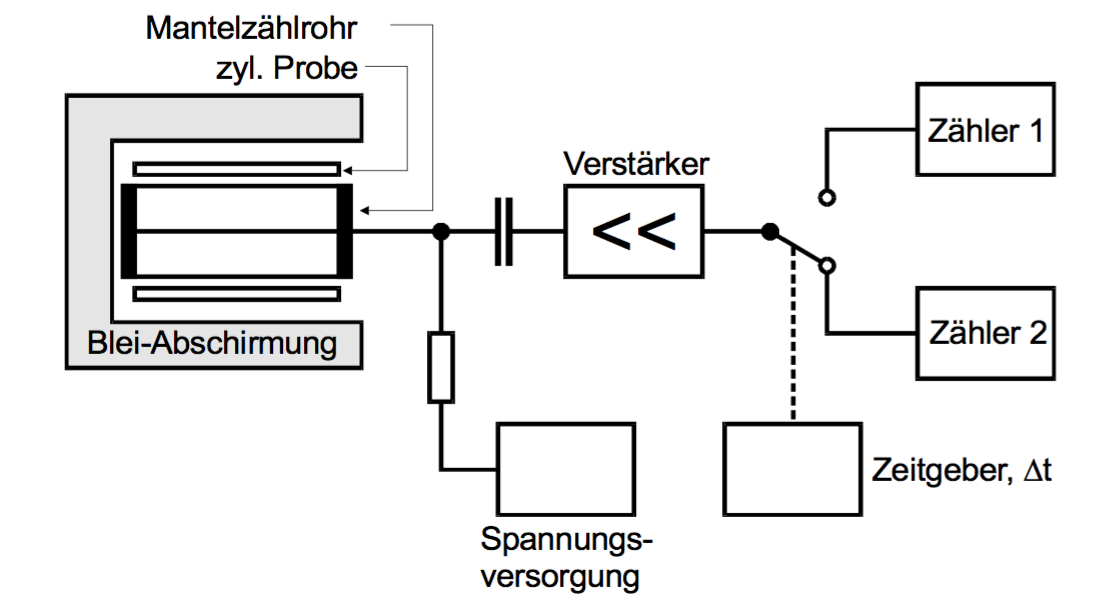
\includegraphics[height=5cm]{Aufbau.png}
  \caption{Versuchsaufbau \cite{skript}.}
  \label{fig:aufbau}
\end{figure}
Die Messapparatur ist in Abbildung \ref{fig:aufbau}
schematisch dargestellt. Das Geiger-Müller-Zählrohr, welches sich in einer Bleiabschirmung
befindet, misst hierbei einen konstanten Anteil der emittierten $\beta^-$-Strahlung.
Damit durchgängig gemessen werden kann, besitzt das Messgerät zwei Anzeigen, zwischen
welchen nach jeder Messung gewechselt wird.\\
Zunächst muss über einen Zeitraum von $\increment\text{t} = \SI{900}{\second}$ der sogenannte
Nulleffekt gemessen werden, also die natürliche radioaktive Strahlung und die Höhenstrahlung,
was bei der Auswertung von jedem Messwert abgezogen werden muss. \\
Bei der Messung von Silber wird an der Messapparatur ein Zeitintervall von $\increment\text{t} = \SI{8}{\second}$
eingestellt und insgesamt 44 Messwerte notiert.
Die Messung von Indium erfolgt bei einem Zeitintervall von $\increment\text{t} = \SI{240}{\second}$
mit 15 Messwertpaaren.
